%!TEX root = ../memoria.tex

\chapter{Figuras}

\section{1}

%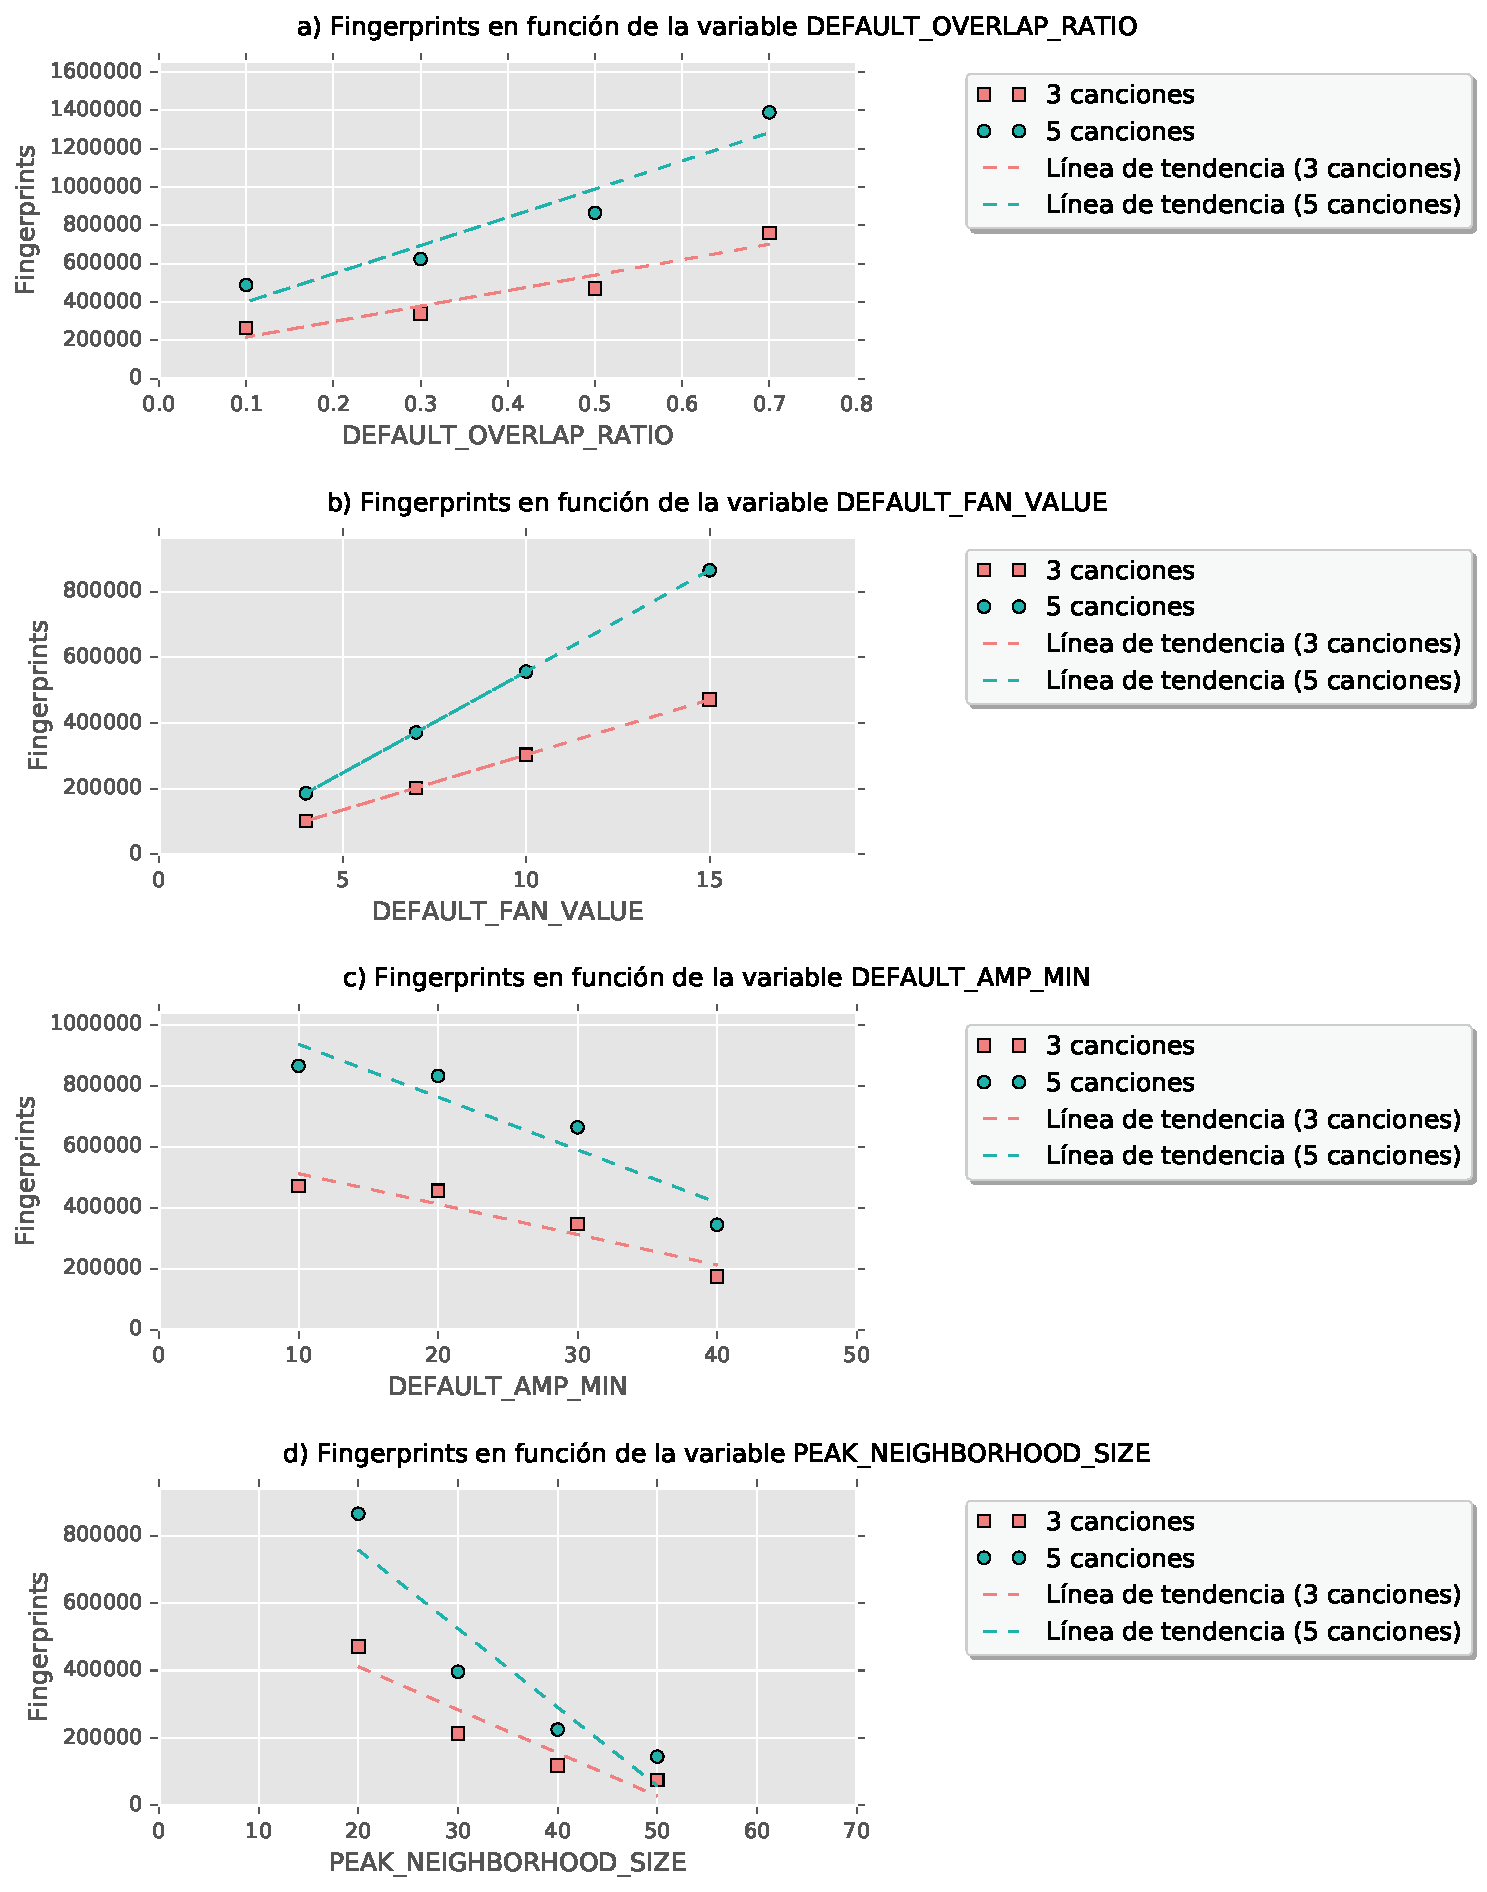
\includepdf[pages=-]{graficos/FingerprintsEnFuncionVariables.pdf}








\begin{figure}[h]
    \centering
    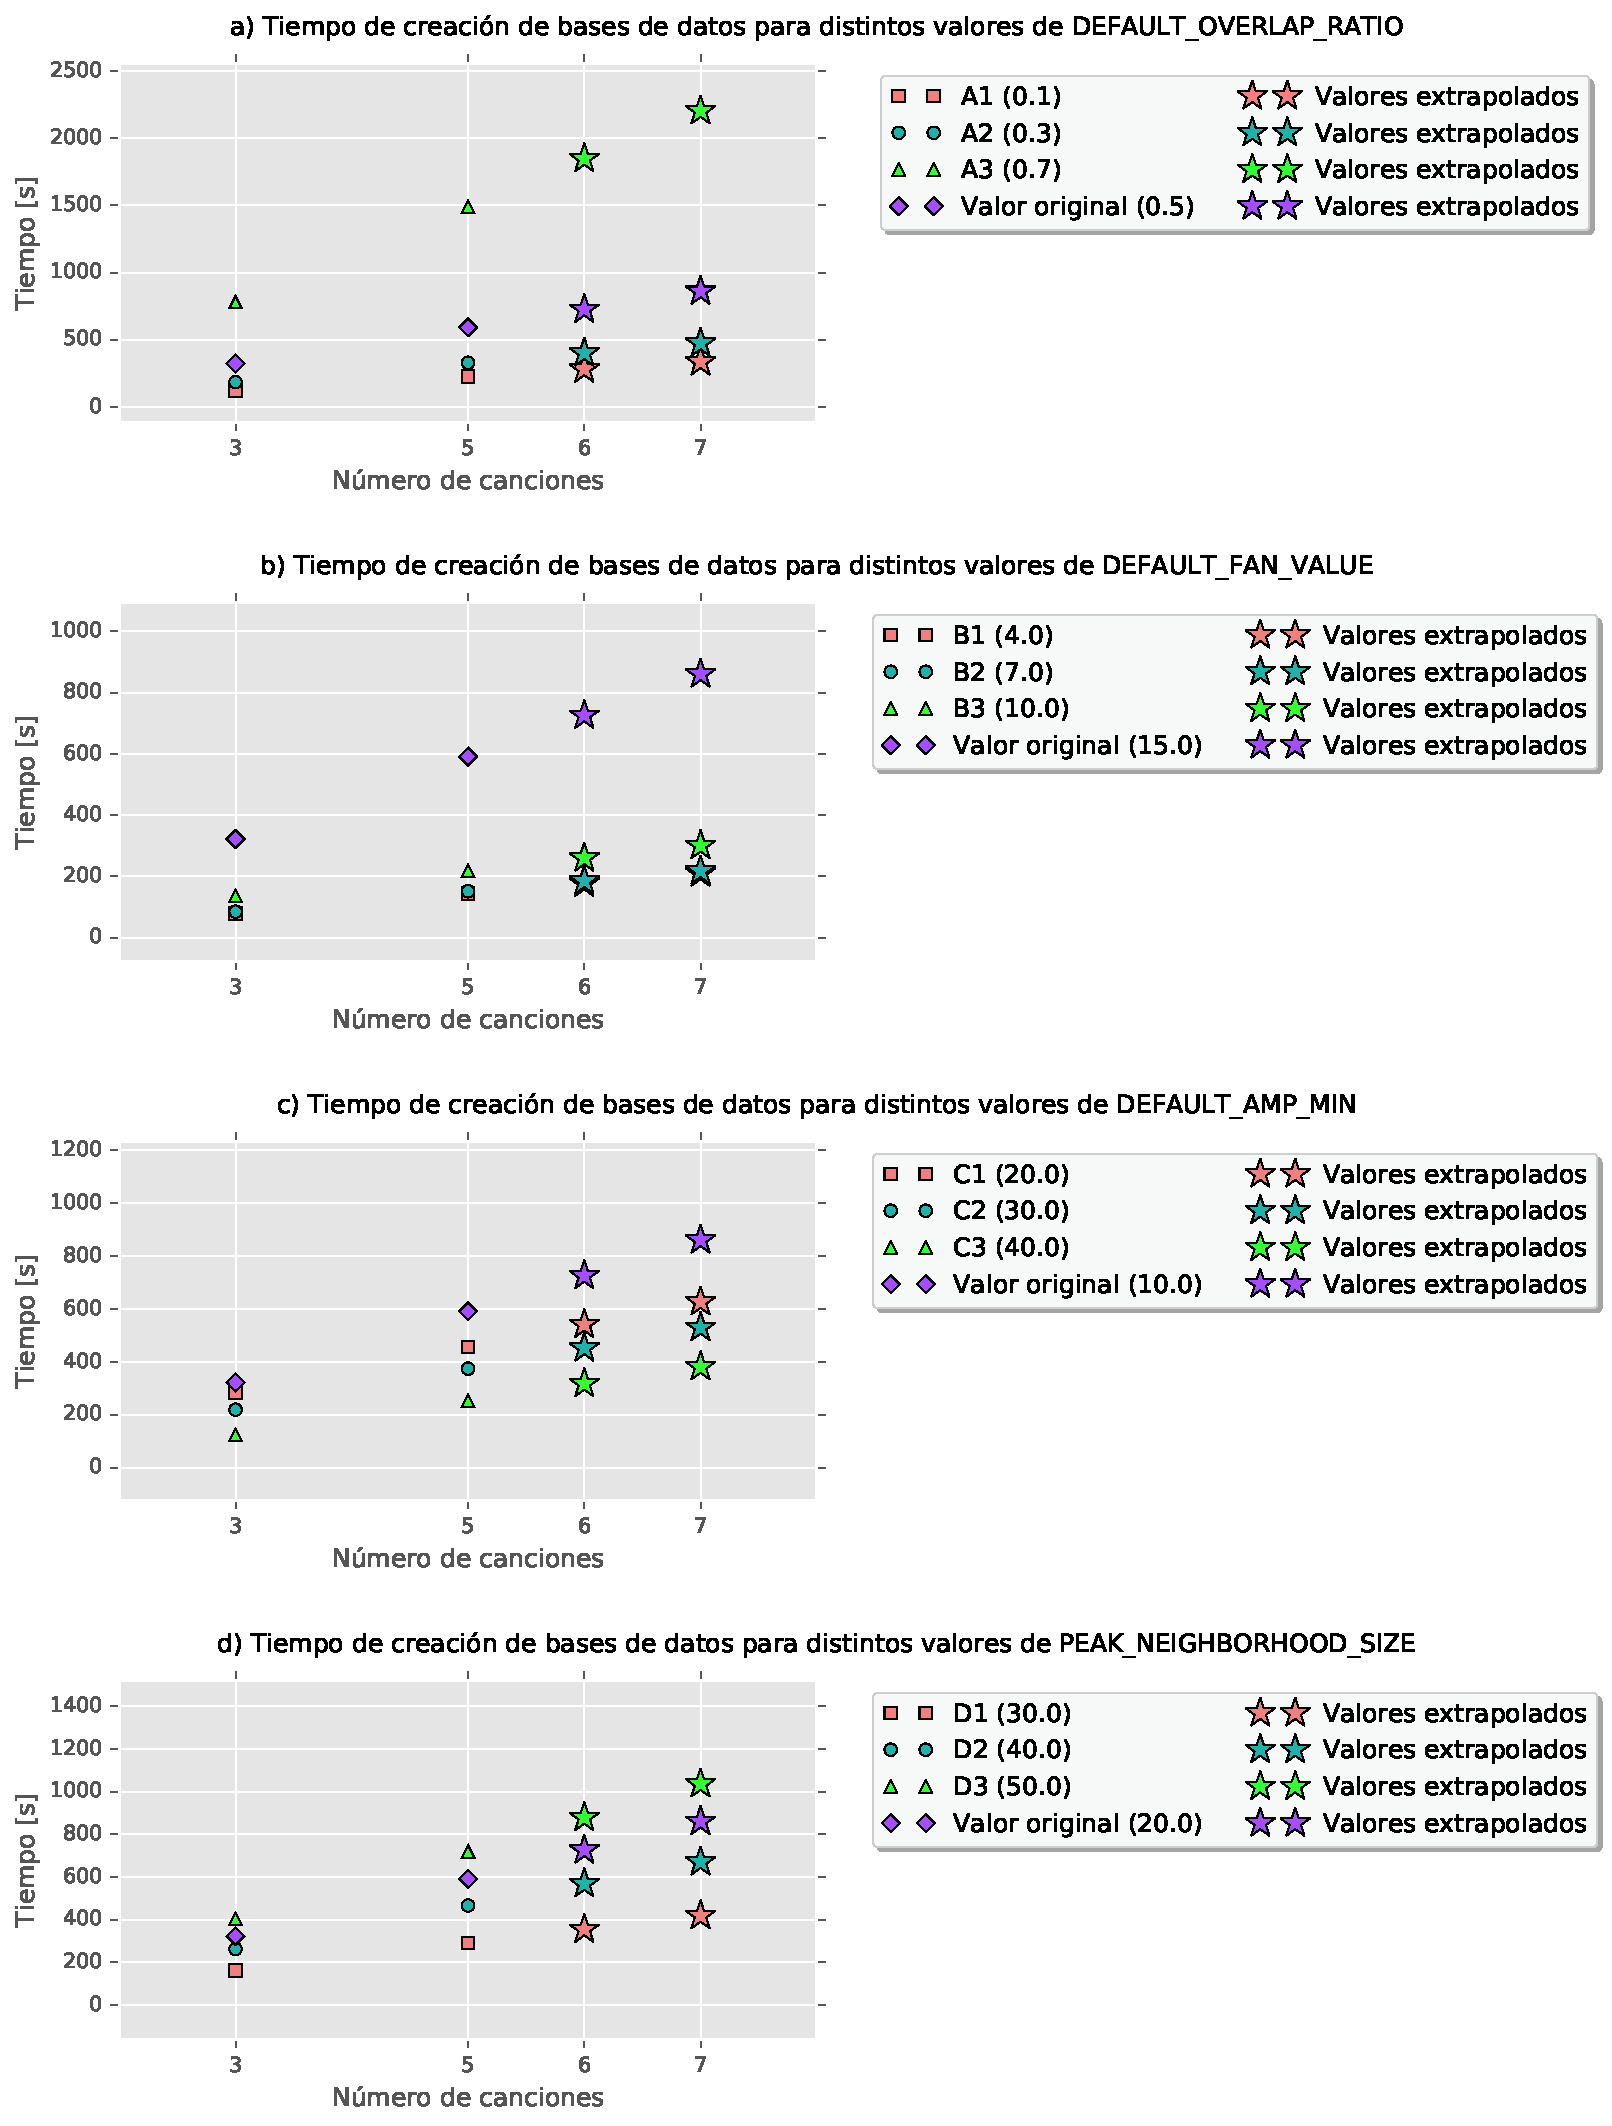
\includegraphics[scale=0.6]{graficos/AnalisisTest35Canciones.pdf}
    \caption{Tiempo de creación de bases de datos al modificar valores de configuración.}{Tiempo transcurrido en la creación de las bases de datos de tres y cinco canciones, con dos valores extrapolados para cada grupo de variables, utilizados para estimar cuanto tardaría una base de datos de 80.000 canciones.}
    \label{fig:AnalisisTest35Canciones}
\end{figure}
Mira mira \ref{fig:AnalisisTest35Canciones}

\begin{figure}[h]
    \centering
    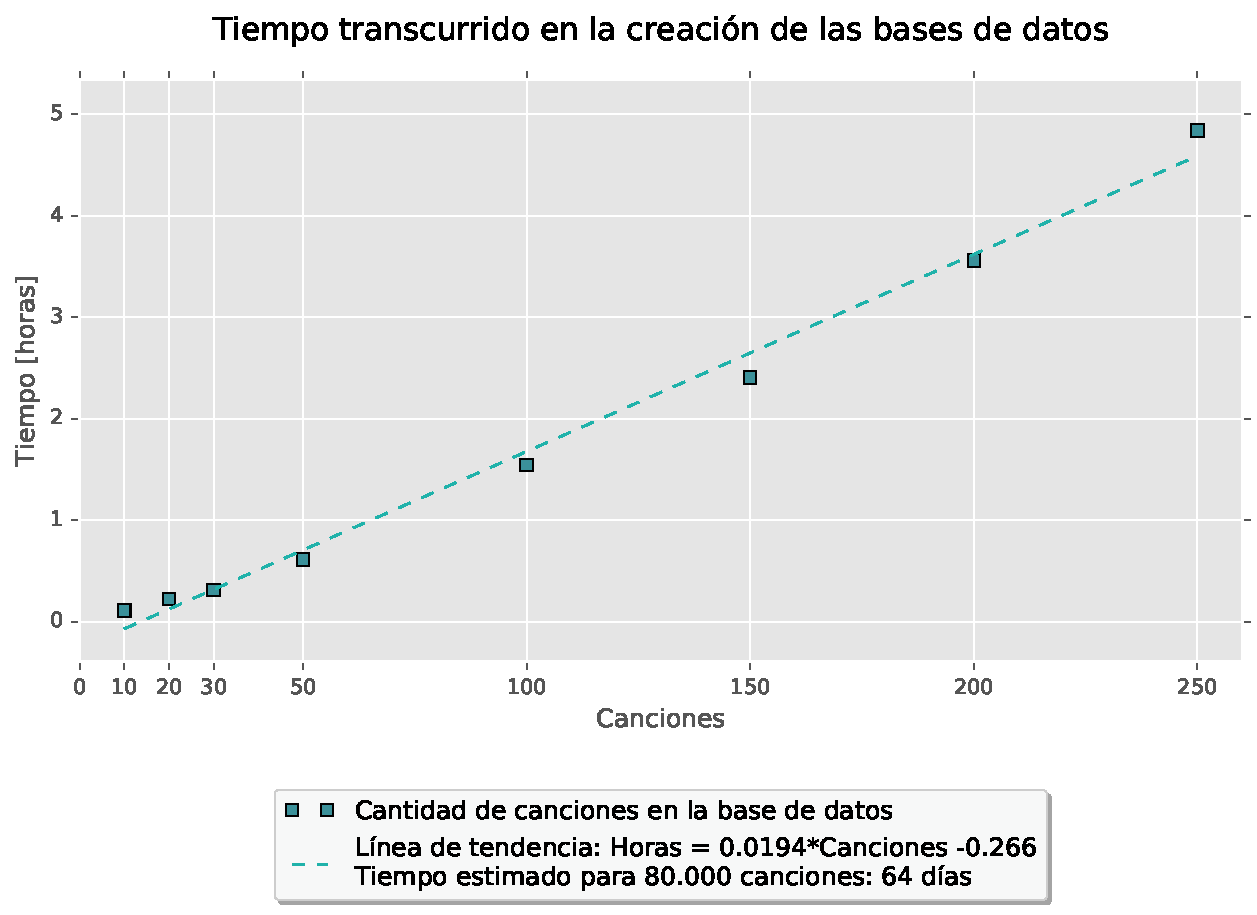
\includegraphics[scale=0.6]{graficos/ExtrapolarTiempoValoresConfiguracion.pdf}
    \caption{Tiempo en función del número de canciones de la nueva configuración de Dejavu.}{Tiempo transcurrido en la creación de las bases de datos con la nueva configuración de Dejavu. La ecuación de la línea de tendencia, permite extrapolar el valor de los días necesarios para crear la base de datos de 80.000 canciones de la plataforma.}
    \label{fig:ExtrapolarTiempoValoresConfiguracion}
\end{figure}
Mira mira \ref{fig:ExtrapolarTiempoValoresConfiguracion}


Mira mira \ref{fig:TiempoFingerprintOriginales}

